\documentclass[a4paper, 11pt]{article}
\usepackage{comment}
\usepackage{lipsum} 
\usepackage{fullpage} %cambiar margen
\usepackage[a4paper, total={7in, 10in}]{geometry}

\usepackage{amssymb,amsthm} 
\usepackage{amsmath}
\newtheorem{theorem}{Theorem}
\newtheorem{corollary}{Corollary}
\usepackage{graphicx}
\usepackage{tikz}
\usetikzlibrary{arrows}
\usepackage{verbatim}
%\usepackage[numbered]{mcode}
\usepackage{float}
\usepackage{tikz}
\usetikzlibrary{shapes,arrows}
\usetikzlibrary{arrows,calc,positioning}
\usepackage{mathpazo} %tipo de letra 
\usepackage[utf8x]{inputenc} %codificación
\usepackage[T1]{fontenc} %digitación de tildes y ñ
\usepackage[spanish]{babel} %paquete de soporte español

\tikzset{
	block/.style = {draw, rectangle,
		minimum height=1cm,
		minimum width=1.5cm},
	input/.style = {coordinate,node distance=1cm},
	output/.style = {coordinate,node distance=4cm},
	arrow/.style={draw, -latex,node distance=2cm},
	pinstyle/.style = {pin edge={latex-, black,node distance=2cm}},
	sum/.style = {draw, circle, node distance=1cm},
}
\usepackage{xcolor}
\usepackage{mdframed}
\usepackage[shortlabels]{enumitem}
\usepackage{indentfirst}
\usepackage{hyperref}

\usepackage{listings}
\lstdefinestyle{customc}{
  belowcaptionskip=1\baselineskip,
  breaklines=true,
  frame=L,
  xleftmargin=\parindent,
  language=Python,
  showstringspaces=false,
  basicstyle=\footnotesize\ttfamily,
  keywordstyle=\bfseries\color{green!40!black},
  commentstyle=\itshape\color{purple!40!black},
  identifierstyle=\color{blue},
  stringstyle=\color{orange},
}

\lstdefinestyle{customasm}{
  belowcaptionskip=1\baselineskip,
  frame=L,
  xleftmargin=\parindent,
  language=[x86masm]Assembler,
  basicstyle=\footnotesize\ttfamily,
  commentstyle=\itshape\color{purple!40!black},
}

\lstset{escapechar=@,style=customc}



\renewcommand{\thesubsection}{\thesection.\alph{subsection}}

\newenvironment{problem}[2][Ejercicio]
{ \begin{mdframed}[backgroundcolor= red!50] \textbf{#1 #2} \\}
	{  \end{mdframed}}

% Define solution environment
\newenvironment{solution}
{\textcolor{blue}{\textbf{\textit{Solución:\\\noindent}}}}


\renewcommand{\qed}{\quad\qedsymbol}

% \\	
\begin{document}
	\noindent
	%%%%%%%%%%%%%%%%%%%%%%%%%%%%%%%%%%%%
	
	\begin{minipage}[b][1.2cm][t]{0.8\textwidth}
		\large\textbf{César Isaí García Cornejo} \hfill \textbf{Tarea 4}  \\
		cesar.cornejo@cimat.mx \hfill \\
		\normalsize Ciencia de Datos \hfill Semestre 3\\
	\end{minipage}
	
	\hspace{14.4cm}
	\begin{minipage}[b][0.03cm][t]{0.12\linewidth}
		
		\vspace{-2.2cm}
		%%%La Ruta depeendera de donde este alojado el main y la imagen
		
\includegraphics[scale=0.3]{Images/EscudoCimat.png}
	\end{minipage}
	
	\noindent\rule{7in}{2.8pt}
	
	%%%%%%%%%%%%%%%%%%%%%
	%%%%%%%%%%%%%%%%%%%%%%%%%%%%%%%%%%%%%%%%%%%%%%%%%%%%%%%%%%%%%%%%%%%%%%%%%%%%%%%%%%%%%%%%%%%%%%%%%%%%%%%%%%%%%%%%%%%
	% Problem 1
	%%%%%%%%%%%%%%%%%%%%%%%%%%%%%%%%%%%%%%%%%%%%%%%%%%%%%%%%%%%%%%%%%%%%%%%%%%%%%%%%%%%%%%%%%%%%%%%%%%%%%%%%%%%%%%%%%%%%%%%%%%%%%%%%%%%%%%%%
	\setlength{\parskip}{\medskipamount}
	\setlength{\parindent}{0pt}
 
\begin{problem}{1} 
    Retomemos el conjunto de datos Iris que podemos llamar gracias a la función \textit{load\_iris} del paquete \textit{sklearn.datasets}. En estudios de datos anteriores vimos que las dos variables \textit{petal length} y \textit{petal width} son muy correlacionadas con las categorías de las plantas.
    \begin{enumerate}[a)]
        \item Usando los datos bidimensionales correspondientes a \textit{petal length} y \textit{petal width} de cada planta, observar el resultado del clustering \textit{k-medias} de los datos con 2,3 y 4 clases. Se usará la función \textit{KMeans} de \textit{sklearn.cluster}.
        \item Escribir una función \textit{Riesgo}(X,y,C) que toma los datos $X$, las categorías correspondientes y los centroides $C$ y que responde el valor de la función $G$ (definida en el curso).
        \item Graficar el resultado de \textit{Riesgo} para $k$ que varia entre 2 y 10. 
        \item Para elegir el mejor $k$ una técnica famosa el la \textit{Elbow Method}. Hacer una búsqueda de referencias que explican la técnica. Implementar la técnica para la grafica del inciso anterior.
    \end{enumerate}

\end{problem}



\begin{solution} 
    \begin{enumerate}[a)]
        \item Usaremos los datos de Iris correspondientes a lo largo y ancho del pétalo. Dichos datos con la clasificación predeterminada de la base de datos (a priori) se observan en el siguiente gráfico
        \begin{figure}[H] 
            \centering 
            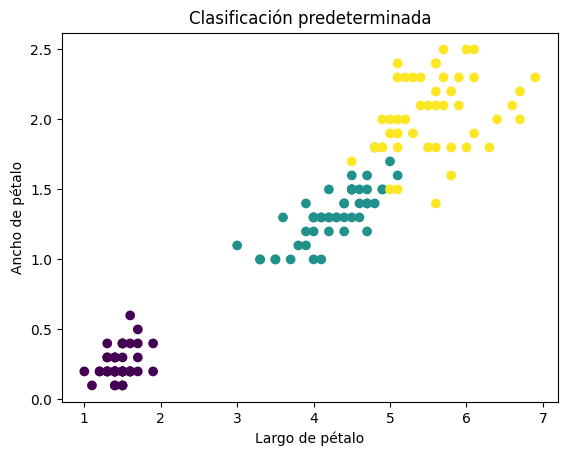
\includegraphics[width = 10 cm ]{Images/iris.png} 
            \caption{Largo y ancho de los pétalos en la base de datos Iris.}
            \label{Fig. 1.01}
        \end{figure} 

        Entonces, ocultaremos la etiqueta de las clases para proceder a Implementar el método de k-means con la paquetería requerida. Ampliamente hablando, la implementación fundamental está en el código
        \begin{lstlisting}
kmeans = KMeans(n_clusters=n)
kmeans.fit(X)
y_kmeans = kmeans.fit_predict(X)
        \end{lstlisting}
        donde $n$ es el número de cluster fijado por el experimentador.

        Así, dicha clusterización para 2,3 y 4 clases se muestan en las graficamente en las siguientes figuras.
        \begin{figure}[H] 
            \centering 
            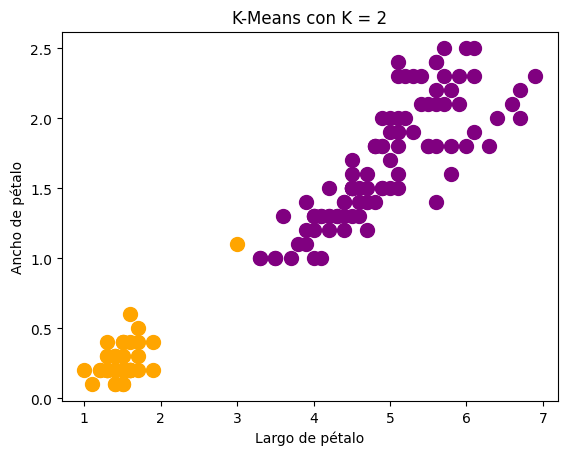
\includegraphics[width = 10 cm ]{Images/clus2.png} 
            \caption{Método de k-means para 2 clusters.}
            \label{Fig. 1.02}
        \end{figure} 

        \begin{figure}[H] 
            \centering 
            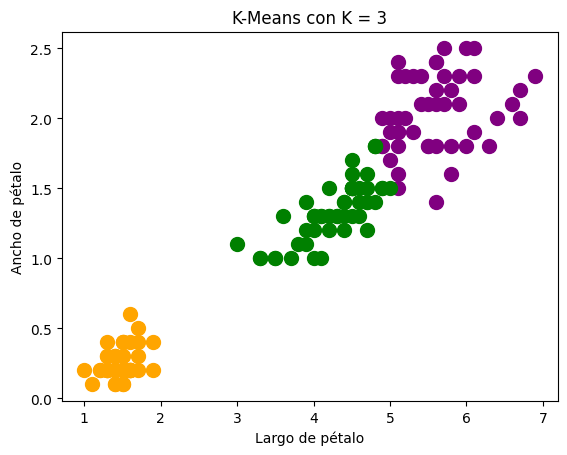
\includegraphics[width = 10 cm ]{Images/clus3.png} 
            \caption{Método de k-means para 3 clusters.}
            \label{Fig. 1.03}
        \end{figure} 
        \begin{figure}[H] 
            \centering 
            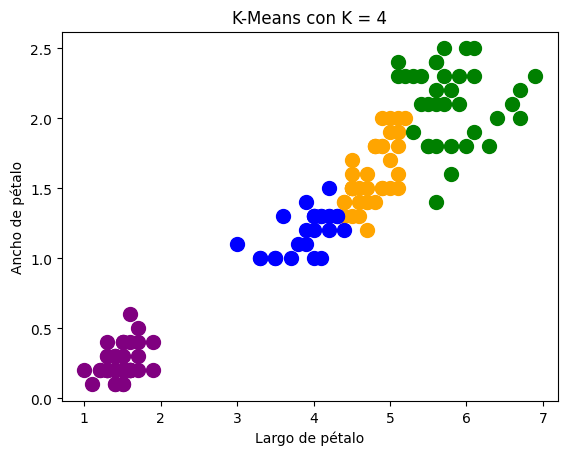
\includegraphics[width = 10 cm ]{Images/clus4.png} 
            \caption{Método de k-means para 4 clusters.}
            \label{Fig. 1.04}
        \end{figure} 

        El código completo está anexo en la actividad correspondiente.

        \item La función de riesgo implementada se basa en usar DataFrames de pandas para que una vez hecha la clusterización podamos filtrar aquellos datos que pertenecen a la misma clase y poder calcular su centroide. Luego, calculamos el cuadrado de la distancia y sumamos obteniendo el riesgo para dicha clase. Hacemos lo mismo para cada clase y sumamos. 
        
        La implementación es
        \begin{lstlisting}
def riesgo(X,k):
    # Base de datos
    df = pd.DataFrame(X, columns=['Largo', 'Ancho'])

    kmeans = KMeans(n_clusters=k)
    kmeans.fit(X)
    y_kmeans = kmeans.fit_predict(X)
    df['Cluster'] = y_kmeans

    riesgo = 0
    for i in range(n):

        #Filtrar por clase i
        d0 = df[df['Cluster'] == i]

        #Calculo de la media
        x = d0['Largo']-d0['Largo'].mean()
        y = d0['Ancho']-d0['Ancho'].mean()

        # plt.plot(d0['Largo'].mean(), d0['Ancho'].mean(), '*k') #plot
        dist = (x**2 + y**2).sum()
        riesgo += dist
        # print(dist)

    return riesgo
        \end{lstlisting}

        \item Hacemos un ciclo para k, los valores entre 2 y 10, con el fin de que podamos calcular el riesgo con el método de k-means para cada valor de k dentro del ciclo. Dicho resultado nos dá la siguiente grafica
        \begin{figure}[H] 
            \centering 
            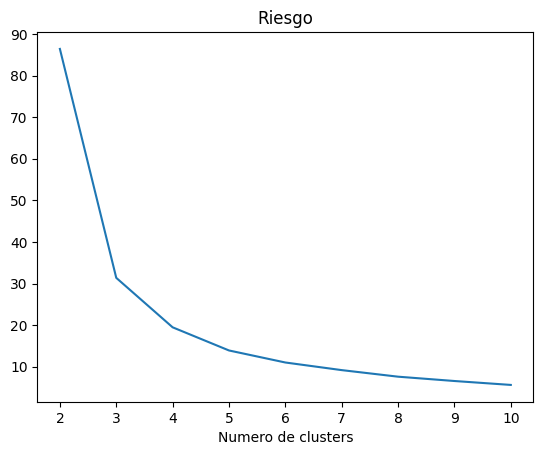
\includegraphics[width = 10 cm ]{Images/riesgo.png} 
            \caption{Riesgo dado por el método de K-means con k clusters.}
            \label{Fig. 1.05}
        \end{figure} 


        \item Por último la interpretación dada a la gráfica anterior con el método del codo, observamos donde el riesgo cambia de forma que aparenta un ángulo de 90 grados, que como podemos observar este valor se da en k = 3. Es decir, el valor óptimo de cluster es 3, que se corresponde con el etiquetado correcto.
    \end{enumerate}

\end{solution}




\end{document}